
%=============================================================================
%  File:          main.tex
%  Author:        Holger Junker
%                 Electronics Lab, ETH Zurich, Switzerland
%                 junker(at)ife.ee.ethz.ch
%  Content:       Template for student reports
%  Creation:      11 Jan 2001
%  Last change:   continuous ...
%=============================================================================
%\newif\ifpdf
%\ifx\pdfoutput\undefined
%  \pdffalse
%\else
%  \pdfoutput=1
%  \pdftrue
%\fi	

\RequirePackage{ifpdf}

\ifpdf



%\RequirePackage{ifpdf}
%\documentclass{JHEP3}

\documentclass[11pt,            % 11pt Font
               a4paper,         % a4-Paperformat
               twoside,         % twoside
               fleqn,           % Equations appear flush left
               pdftex
               ]{report}
\else
\documentclass[11pt,            % 11pt Font
               a4paper,         % a4-Paperformat
               twoside,         % twoside
               fleqn,           % Equations appear flush left
               openright        % Chapters begin on odd (right) page
              ]{report}
\fi


\ifpdf
     \usepackage[colorlinks,hyperindex]{hyperref}% generates colored links
                                                 % in pdf file
     \usepackage[pdftex]{graphicx}
     \DeclareGraphicsExtensions{.png, .jpg, .pdf}
     \graphicspath{{pictures/}}
\else
     \usepackage[dvips]{graphicx}
     \DeclareGraphicsExtensions{.eps}
     \graphicspath{{pictures/}}
\fi

\usepackage[T1]{fontenc}        % T1-Fontcoding, auch notwendig
                                % um mit Umlauten �,�,� arbeiten zu koennen
\usepackage{ae}                 % Almost european computer modern font
                                % Zur Erstellung von pdf-Files
\usepackage[english]{babel}      % Package for multilingual style options
\usepackage{fancyhdr}           % Package for customizing page layout
\usepackage{ETHkopfTwo}         % ETH Style Title page
\usepackage{AufgTwo}            % Formatiert die Aufgabenstellung
\usepackage{verbatim}           % Package for including files


%=============================================================================
% Layout Header and Footer
%=============================================================================

\pagestyle{fancy}
% with this we ensure that the chapter and section
% headings are in lowercase.
\renewcommand{\chaptermark}[1]{\markboth{\thechapter\ #1}{}}
\renewcommand{\sectionmark}[1]{\markright{\thesection\ #1}}
\fancyhf{}                           % Delete all current settings
                                     % for header and footer
\fancyhead[LE,RO]{\bfseries\thepage} % Pagenumber aligned left on odd pages
                                     % Pagenumber aligned right on
                                     % even pages
\fancyhead[LO]{\nouppercase{\bfseries\rightmark}}
\fancyhead[RE]{\nouppercase{\bfseries\leftmark}}
\renewcommand{\headrulewidth}{0.5pt}
\renewcommand{\footrulewidth}{0pt}
\addtolength{\headheight}{1.6pt}     % Make space for headrule
\fancypagestyle{plain}
{
\fancyhead{}                         % Get rid of headers on plain pages
\renewcommand{\headrulewidth}{0pt}   % Get rid of headerline on plain pages
}

%=============================================================================
% Pagelayout
%=============================================================================

\addtolength{\headwidth}{1.2cm}
\addtolength{\textwidth}{1.2cm}
\addtolength{\evensidemargin}{-1.2cm}
\addtolength{\oddsidemargin}{-0cm}


%=============================================================================
% Numbering depth for headings
%=============================================================================
\setcounter{secnumdepth}{3} % Within document
\setcounter{tocdepth}{3}    % Within table of contents

%=============================================================================
% New commands
%=============================================================================

% These commands may be used instead of the built-in commands of LaTeX
% for creating your equations
\newcommand{\be}{\begin{equation}}          % Abbreviation
\newcommand{\ee}{\end{equation}}
\newcommand{\bea}{\begin{eqnarray}}
\newcommand{\eea}{\end{eqnarray}}


%Command clear used to produce empty page without header and footer
%in case of a twoside report where new chapters always begin on odd pages
\ifpdf
   \newcommand{\clear}{}
\else
   \newcommand{\clear}{\newpage{\pagestyle{empty}\cleardoublepage}}
\fi


\frenchspacing

%=============================================================================
% Begin of document
%=============================================================================

\begin{document}
    \begin{titlepage}
   \pagestyle{empty}
   \topmargin=1.2cm
   \ETHkopfTwo{Wearable Computing Lab}{Prof. G. Troester}{Spring Semester 2014}
   \vspace{-0.5cm}
   \noindent
   \rule{\textwidth}{0 mm}\\

\vspace{\textheight}
\vspace{-3.5cm}
    \noindent
    \rule{\textwidth}{1 mm}\\
    \noindent
    \bfseries \large
    \makebox[0.5\textwidth][l]{\emph{Author:}}
    \makebox[0.49\textwidth][r]{\emph{Supervisors:}}

    \vspace{0.2 cm} \noindent
    \makebox[0.5\textwidth][l]{Frederik Hess}
    \makebox[0.49\textwidth][r]{Long-Van Nguyen-Dinh}
    \makebox[0.5\textwidth][l]{}
    \makebox[0.49\textwidth][r]{Ulf Blanke}

    \mdseries \normalsize


\vspace{-20cm}
\begin{center}
\Large \bfseries Master's Thesis\\
\vspace{0.5cm}
\LARGE \bfseries Interactive Context Recognition in Real-Time Based on Crowdsourced Acoustic Models\\
\end{center}

%Titelbild einf�gen
\begin{center}

\vspace{0.5cm}%Gr�sse ver�ndern zur Positionierung des Bildes

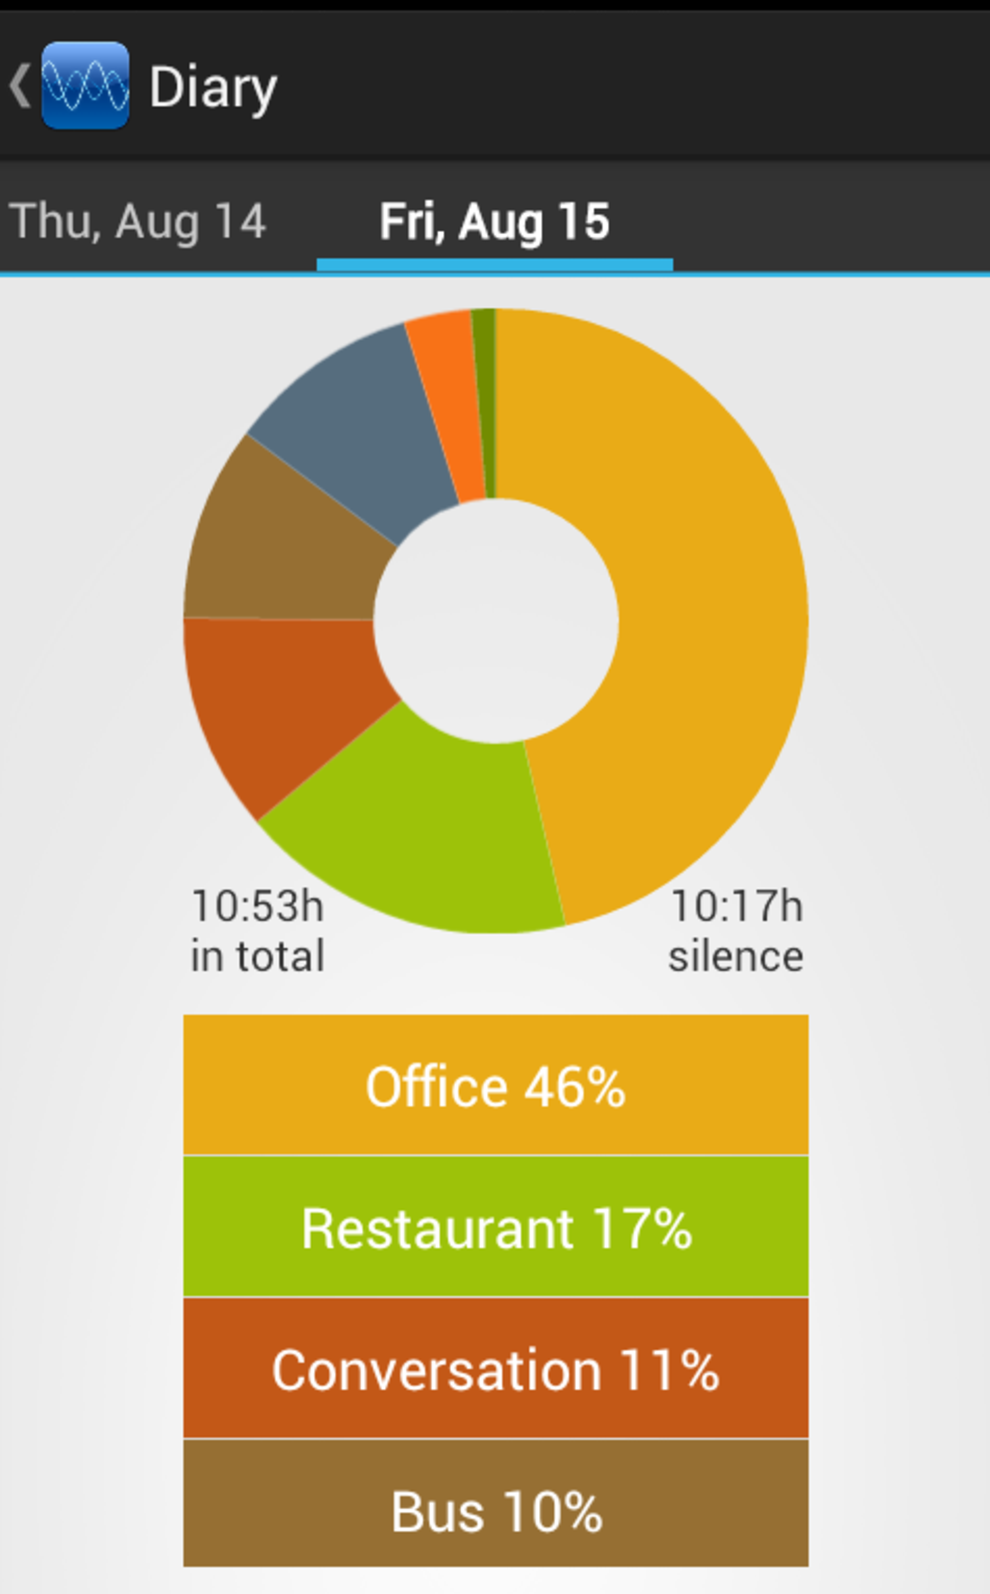
\includegraphics[width=0.5\textwidth]{titelbild}
\end{center}
\end{titlepage}

\clear
    \pagenumbering{roman}

    \chapter*{Preamble}
\addcontentsline{toc}{chapter}{Preamble}
abc\\
\\
\\
By signing this statement, I affirm that I have read the information notice on plagiarism, independently produced this paper, and adhered to the general practice of source citation in this subject-area.
\\
Information notice on plagiarism:
\\
\\
\verb"http://www.ethz.ch/students/exams/plagiarism_s_en.pdf"
\\
\\
\\
\begin{tabbing}
\noindent\rule{4cm}{0.4pt} \hspace{1cm} \noindent\rule{5cm}{0.4pt}
\\
Place and Date \hspace{2.5cm}Signature
\end{tabbing} 
\clear
    \includepdf[pages=-]{Aufgabenstellung.pdf}
\clear
    \tableofcontents
\clear
    \listoffigures % Creates list of all figures used in document
\clear
    \listoftables  % Creates list of all tables inserted
\clear
    \chapter*{Abstract}
\addcontentsline{toc}{chapter}{Abstract}
This is the astract












\clear

% Split your document e.g. chapterwise and rejoin the chapters
% to a single documentation with the \include-Command
    \pagenumbering{arabic}
    \chapter{Introduction}\label{cha1}
\section{Motivation}
Recent technological advances of mobile phone have created the possibility (goal??) to quantitatively (??) predict the context of the user. According to Lane et al. this is mainly the result of the following developments:
\begin{itemize}
  \item The first item
  \item The second item
  \item The third etc \ldots
\end{itemize}


- Increasing performance of mobile platform enables context recognition

- Help understanding human behaviour better (in a quantitative way)

- Improve human-computer interaction (with example)

- Audio modality can give deeper insights than other, more common modalities like only location

-  

\section{Related Work}\label{relatedWork}
bla

\subsection{Audio based context recognition}\label{abc}
abc

\subsection{Crowd-sourcing}
abc

\subsection{Active learning}
abc

\subsection{Gaussian mixture model}
abc








 % TeX includes file Chapter1.tex
\clear
    \chapter{Offline Classification (??)}\label{cha2}
cha2

\section{abc}
abc





\clear
    \chapter{Implementation}\label{cha3}

\section{Classification}

\section{Android Implementation}

\section{Server Back-end Implementation}


\clear
    \chapter{Evaluation}\label{cha4}
abc
\section{abc}

\clear
    \chapter*{Conclusions and Outlook}\label{ausblick}
\addcontentsline{toc}{chapter}{Conclusions and Outlook}
abc




\clear
    \chapter*{Outlook}\label{ausblick}
\addcontentsline{toc}{chapter}{Outlook}
not used
\clear
    %Bibliography
    \bibliographystyle{unsrt}
    \bibliography{bib/example}
\clear

    %Appendix
    \appendix
    % uncomment the following line in case you need to make the page wider
    %\addtolength{\headwidth}{1.2cm}\addtolength{\textwidth}{0.5cm}
    \include{Schematics}
\clear
    \include{Software}
    % uncomment the following line in case you made the page wider earlier
    %\addtolength{\headwidth}{-1.2cm}\addtolength{\textwidth}{-0.5cm}

\end{document}
